\documentclass[12pt,a4paper]{article}
\usepackage[utf8]{inputenc}
\usepackage[T2A]{fontenc}
\usepackage[ukrainian]{babel}
\usepackage{fancyvrb}
\usepackage{pdflscape}

\usepackage{amsmath} % у преамбулі
\usepackage{array, multirow}
\usepackage{hyperref} % <-- Обов’язково підключіть цей пакет
\usepackage{caption}
\usepackage{booktabs}
\usepackage{subcaption} % для підписів (а), (б)
\usepackage{breqn} % Пакет для автоматичного перенесення виразів
\usepackage{mathtools} % Для додаткових можливостей, наприклад, для створення кастомних конструкцій

\usepackage{xcolor}

\renewcommand{\thetable}{№\arabic{table}}
\captionsetup[table]{name=Таблиця}  % замість "Табл." буде "Таблиця"

\usepackage{graphicx} % <-- Для роботи з \includegraphics
\usepackage{geometry}
\geometry{
    left=2cm,
    right=2cm,
    top=2cm,
    bottom=2cm
}


\begin{document}

    \begin{titlepage}

        \thispagestyle{empty}
        \begin{center}
        \large
        Національний технічний університет України\\
        «Київський політехнічний інститут імені Ігоря Сікорського»\\[1em]
        Факультет інформатики та обчислювальної техніки\\
        Кафедра загальної фізики
        \end{center}

        \vfill

        \begin{center}
        \textbf{\LARGE Фізика}\\[2em]
        \textbf{\Large Лабораторна робота №3-3}\\
        «Вивчення дифракції Фраунгофера світла на щілині та дифракційній ґратці» 
        \end{center}

        \vfill

        \begin{flushright}
        Виконав: студент 1 курсу ФІОТ, гр. ІО-41\\
        \textit{Давидчук А. М.}\\
        Залікова книжка № 4106\\[1em]
        Перевірив: \textit{Колган В.\,В.}
        \end{flushright}

        \vfill

        \begin{center}
        Київ -- 2025
        \end{center}

    \end{titlepage}

    \setlength{\parindent}{0pt}

    \textbf{\underline{Тема:}} «Вивчення дифракції Фраунгофера світла на щілині та дифракційній ґратці».

    \vspace{1em}

    \textbf{\underline{Мета:}} експериментально вивчити залежність інтенсивності світла від
    кутів дифракції, визначити довжину хвилі випромінювання.

    \vspace{1.5em}

    \begin{center} \textbf{\Large Теоретичні відомості} \end{center}
    \setlength{\parindent}{1.5em}

    \begin{center} \textbf{Дифракція плоскої монохроматичної хвилі на щілині} \end{center}

    Якщо на довгу вузьку щілину нормально падає плоска монохроматична хвиля, то розподіл інтенсивності світла на екрані залежно від відстані до центра
    щілини задається функцією:

    \begin{equation}
        I(\varphi) = I_0 \left( \frac{\sin(\pi b \lambda^{-1} \sin \varphi)}{\pi b \lambda^{-1} \sin \varphi} \right)^2,
        \tag{3.1}
    \end{equation}

    графік якої представлений на рис. (3.1):

    \begin{figure}[!ht]

        \renewcommand{\thefigure}{3.\arabic{figure}} % робимо "3.1", "3.2" і т.д.

        \centering
        % Підставляєте потрібний шлях та розмір зображення:
        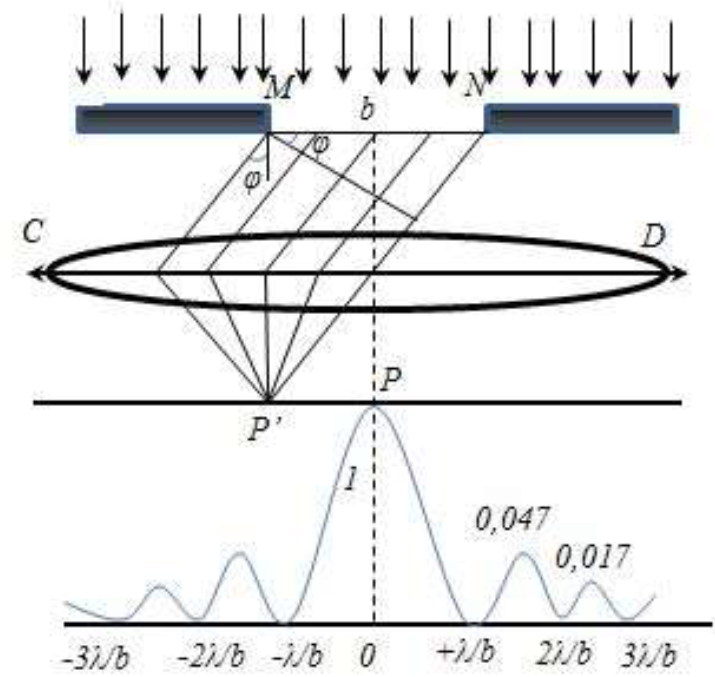
\includegraphics[width=0.3\textwidth]{3.1.png}
        % Підпис (зазвичай під малюнком):
        \caption{}
        % Мітка для посилань у тексті (\ref{fig:...})
        \label{fig1:schema}

    \end{figure}

    У формулі (3.1) $I_0$ --- інтенсивність хвилі, що падає, $\lambda$ --- довжина хвилі, $b$ --- ширина щілини.

    У розподілі можна виділити центральний максимум при $\varphi = 0$ та ряд побічних максимумів, напрямки на які залежно від кута $\varphi$ відхилення
    променів знаходиться за умовою:

    \begin{equation}
        b\varphi \approx \pm \left( 2n + 1 \right) \frac{\lambda}{2},
        \tag{3.2}
    \end{equation}

    де $n = 0, 1, 2, \dots$.
    Умова спостереження мінімумів, що розділяють максимуми:
    \[
    b\sin \varphi = \pm n \lambda,
    \]

    або для малих кутів:

    \begin{equation}
        b\varphi = \pm n \lambda.
        \tag{3.3}
    \end{equation}

    З умов екстремумів виходить, що зменшення ширини щілини призводить до
    збільшення відстані між мінімумами, тобто до розширення дифракційної
    картини.

    Якщо $b = \lambda$, то центральний максимум розпливається на весь екран ($\varphi_{min} = \arcsin 1$)
    і подальше зменшення $b$ позбавлено сенсу у зв'язку із зникненням
    структури дифракційній картині. Збільшення ширини щілини призводить до
    звуження дифракційної картини. Максимально припустима ширина щілини $b_{max}$
    визначається роздільною здатністю ока.
    Прирівнюючи кутове положення першого мінімуму найменшій роздільній здатності
    ока (у кутових одиницях) $\lambda \slash b_{max} \approx 10^{-3}$, бачимо,
    що $b_{max} \approx 10^3 \lambda$. Таким чином, під час спостереження
    дифракції світла на щілині її ширина повинна знаходитись у межах $\lambda \leq b \leq 10^3 \lambda$
    (наприклад, для видимого світла $0,5 \leq b \leq 500 \text{мкм}$).
    Аналіз виразу (3.1) пояснює й інші особливості дифракційної картини.

    \begin{center} \textbf{Дифракція плоскої монохроматичної хвилі на ґратці} \end{center}

    У науці та техніці широко використовується дифракція світла на системі
    паралельних, розташованих на однаковій відстані щілинах, так званій
    дифракційній ґратці (решітці).

    Якщо на ґратку нормально падає монохроматичне світло (рис. 3.2),
    
    \begin{figure}[!ht]

        \renewcommand{\thefigure}{3.\arabic{figure}} % робимо "3.1", "3.2" і т.д.

        \centering
        % Підставляєте потрібний шлях та розмір зображення:
        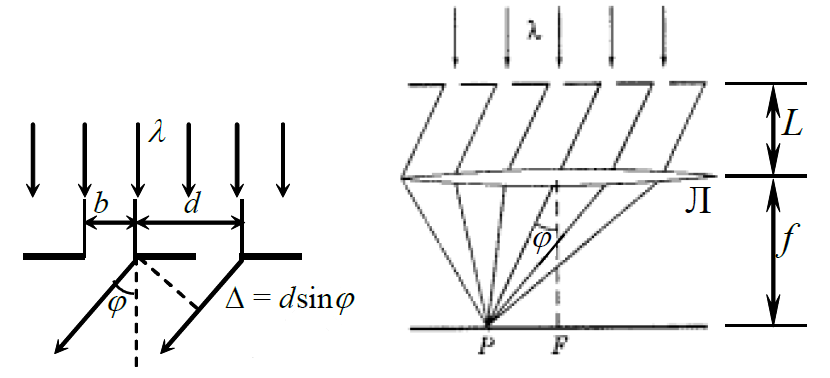
\includegraphics[width=0.5\textwidth]{3.2.png}
        % Підпис (зазвичай під малюнком):
        \caption{}
        % Мітка для посилань у тексті (\ref{fig:...})
        \label{fig2:schema}

    \end{figure}
    
    то розподіл інтенсивності світла описується функцією

    \begin{equation}
        \displaystyle I = I_0 \dfrac{\sin^2 \left( \dfrac{\pi b}{\lambda} \sin \varphi \right)}{\left( \dfrac{\pi b}{\lambda} \sin \varphi \right)^2} \cdot \dfrac{\sin^2 \left( \dfrac{N\pi d}{\lambda} \sin \varphi \right)}{\sin^2 \left( \dfrac{\pi d}{\lambda} \sin \varphi \right)},
        \tag{3.4}
    \end{equation}

    графік якої схематично представлений на рис. 3.3.

    \begin{figure}[!ht]

        \renewcommand{\thefigure}{3.\arabic{figure}} % робимо "3.1", "3.2" і т.д.

        \centering
        % Підставляєте потрібний шлях та розмір зображення:
        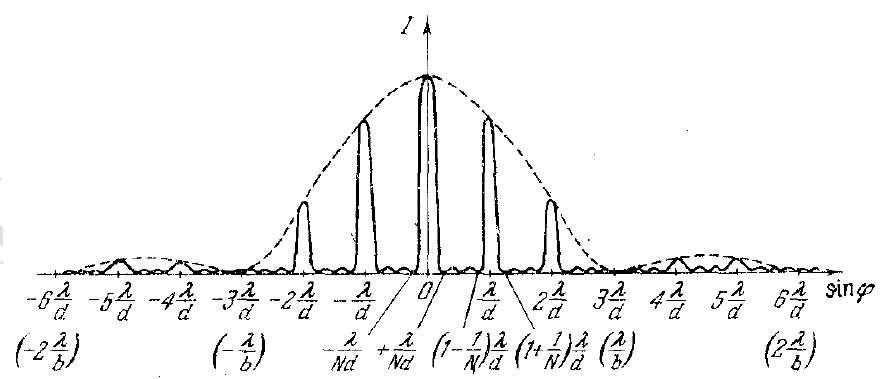
\includegraphics[width=0.5\textwidth]{3.3.png}
        % Підпис (зазвичай під малюнком):
        \caption{}
        % Мітка для посилань у тексті (\ref{fig:...})
        \label{fig3:schema}

    \end{figure}

    Умова спостереження головних максимумів інтенсивності має вигляд

    \begin{equation}
        d \sin \varphi = \pm m\lambda, \quad m = 0, 1, 2, \dots,
        \tag{3.5}
    \end{equation}

    де $d$ – період дифракційної ґратки, який дорівнює сумі ширини прозорої та
    непрозорої частин (див. рис. 3.2).

    \newpage

    \begin{center} \textbf{\Large Практична частина} \end{center}

    \begin{center} \textbf{Опис експериментальної установки та методика вимірювань} \end{center}

    Схема експериментальної установки показана на рис. З.4.

    \begin{figure}[!ht]

        \renewcommand{\thefigure}{3.\arabic{figure}} % робимо "3.1", "3.2" і т.д.

        \centering
        % Підставляєте потрібний шлях та розмір зображення:
        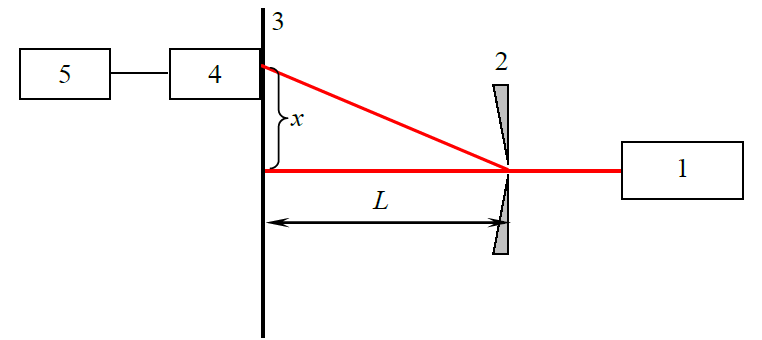
\includegraphics[width=0.5\textwidth]{3.4.png}
        % Підпис (зазвичай під малюнком):
        \caption{}
        % Мітка для посилань у тексті (\ref{fig:...})
        \label{fig4:schema}

    \end{figure}

    Джерелом світла у
    даній роботі є Не-Ne лазер 1, що генерує практично плоску монохроматичну
    хвилю у червоній ділянці спектра. Світлова хвиля направляється на розсувну
    щілину 2 перпендикулярно до її площини. Щілина має мікрогвинт, за допомогою
    якого можна встановлювати потрібну ширину.

    Дифракційна картина спостерігається на екрані 3. У площині екрана можна
    зміщувати фотоприймач 4 з малим вхідним отвором. Сигнал із фотоприймача
    (фотоприймачем є фотодіод), пропорційний середній інтенсивності світла, що
    пройшло крізь вхідний отвір, після підсилення вимірюється вольтметром 5.

    Якщо підібрати ширину щілини 2 так, щоб ширина дифракційного
    максимуму була набагато більшою за розмір вхідного отвору фотоприймача, то за
    допомогою такої експериментальної установки можна достатньо точно виміряти
    розподіл інтенсивності $I(\varphi)$ пучка, що дифрагував і, відповідно, експериментально
    перевірити вираз (3.1).

    Для спостереження дифракії на ґратці її ставлять на місце щілини.

    \textbf{УВАГА!} Категорично забороняється спостерігати світловий пучок, направлений
    безпосередньо від лазера на око або після його відбивання дзеркальною
    поверхнею, тому що це є небезпечним для зору. Лазерний пучок можна
    спостерігати лише розсіяним на не дзеркальних поверхнях (аркуш паперу тощо).

    \begin{center} \textbf{Порядок виконання} \end{center}
    
    \dots

\end{document}